\documentclass[aspectratio=169]{beamer}
\usetheme{metropolis}           % Use metropolis theme
\metroset{numbering=fraction}
\usepackage{tikz}
\usetikzlibrary{positioning}
\usetikzlibrary{arrows,backgrounds,automata,decorations.shapes,decorations.pathmorphing,decorations.markings,decorations.text,positioning,shapes.geometric}

\tikzstyle{place}=[circle,draw=blue!50,fill=blue!20,thick, inner sep=0pt,minimum size=6mm]
\tikzstyle{transition}=[rectangle,draw=black!50,fill=black!20,thick, inner sep=0pt,minimum size=4mm]

\tikzstyle{block}=[rectangle,draw=black, thick, inner sep=5pt]
\tikzstyle{bullet}=[circle,draw=black, fill=black, thin, inner sep=2pt]

\tikzstyle{pre}=[<-,shorten <=1pt,>=stealth',semithick]
\tikzstyle{post}=[->,shorten >=1pt,>=stealth',semithick]
\tikzstyle{bi}=[<->,shorten >=1pt,shorten <=1pt, >=stealth',semithick]

\tikzstyle{mut}=[-,>=stealth',semithick]

\tikzstyle{treereset}=[dashed,->, shorten >=1pt,>=stealth',thin]

\pgfdeclarelayer{edgelayer}
\pgfdeclarelayer{nodelayer}
\pgfsetlayers{edgelayer,nodelayer,main}

\tikzstyle{none}=[inner sep=0pt]
\tikzstyle{rn}=[circle,fill=Red,draw=Black,line width=0.8 pt]
\tikzstyle{gn}=[circle,fill=Lime,draw=Black,line width=0.8 pt]
\tikzstyle{yn}=[circle,fill=Yellow,draw=Black,line width=0.8 pt]
\tikzstyle{empty}=[circle,fill=White,draw=Black]
\tikzstyle{bw} = [rectangle, draw, fill=blue!20, 
    text width=4em, text centered, rounded corners, minimum height=2em]

\usepackage{float}
\usepackage{makecell}
\usepackage{fancyvrb}
\usepackage{listings}
\usepackage[export]{adjustbox}
\usepackage{caption}
\usepackage{alltt}
\title{Lecture 4 \\ Java I/O, Event-Driven Programming, Android Sensor Manager}
\date{May 12, 2016}
\author{Patrick Lam \\ Jeff Zarnett \\ Michael Giannikouris}
\institute{Department of Electrical and Computer Engineering}
\setbeamertemplate{caption}{\raggedright\insertcaption\par}
\setbeamersize{text margin left=12pt,text margin right=12pt}
\newcommand{\putat}[3]{\begin{picture}(0,0)(0,0)\put(#1,#2){#3}\end{picture}} % just a shorthand

\newenvironment{deflist}
{ \begin{description}
    \setlength{\itemsep}{6pt}
    \setlength{\parskip}{0pt}
    \setlength{\parsep}{0pt}     }
{ \end{description}              } 

\newenvironment{splitslide}
{
\centering
\begin{tabular}{@{}p{0.50\textwidth} | p{0.025\textwidth}@{} p{0.4\textwidth}@{}}
}
{
\end{tabular}
}


\begin{document}
\maketitle



\section*{Java I/O}



%%%%%%%%%%%%%%%%%%%%%%%%%%%%%%%%%%%%%%%%%%%%%%%%%%%%%%%%%%%%%%%%%%%%%%%%%%%%%%%%%%%%
% Java Input/Output
%%%%%%%%%%%%%%%%%%%%%%%%%%%%%%%%%%%%%%%%%%%%%%%%%%%%%%%%%%%%%%%%%%%%%%%%%%%%%%%%%%%%
\begin{frame}{Java Input/Output}
In Java, Input/Output (or I/O) is modelled as a \textit{Stream}. \\
A Stream is a sequence of data. \\
A stream can be used to read data (input stream) or write data (output stream). \\
\end{frame}
%%%%%%%%%%%%%%%%%%%%%%%%%%%%%%%%%%%%%%%%%%%%%%%%%%%%%%%%%%%%%%%%%%%%%%%%%%%%%%%%%%%%



%%%%%%%%%%%%%%%%%%%%%%%%%%%%%%%%%%%%%%%%%%%%%%%%%%%%%%%%%%%%%%%%%%%%%%%%%%%%%%%%%%%%
% InputStream
%%%%%%%%%%%%%%%%%%%%%%%%%%%%%%%%%%%%%%%%%%%%%%%%%%%%%%%%%%%%%%%%%%%%%%%%%%%%%%%%%%%%
\begin{frame}{InputStream}
\begin{center}
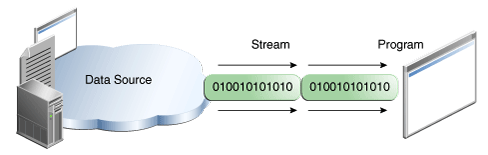
\includegraphics[width=0.85\textwidth]{img/inputstream.png}
\end{center}
\end{frame}
%%%%%%%%%%%%%%%%%%%%%%%%%%%%%%%%%%%%%%%%%%%%%%%%%%%%%%%%%%%%%%%%%%%%%%%%%%%%%%%%%%%%



%%%%%%%%%%%%%%%%%%%%%%%%%%%%%%%%%%%%%%%%%%%%%%%%%%%%%%%%%%%%%%%%%%%%%%%%%%%%%%%%%%%%
% OutputStream
%%%%%%%%%%%%%%%%%%%%%%%%%%%%%%%%%%%%%%%%%%%%%%%%%%%%%%%%%%%%%%%%%%%%%%%%%%%%%%%%%%%%
\begin{frame}{OutputStream}
\begin{center}
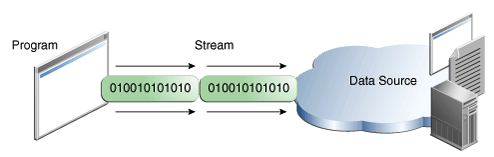
\includegraphics[width=0.85\textwidth]{img/outputstream.png}
\end{center}
\end{frame}
%%%%%%%%%%%%%%%%%%%%%%%%%%%%%%%%%%%%%%%%%%%%%%%%%%%%%%%%%%%%%%%%%%%%%%%%%%%%%%%%%%%%



%%%%%%%%%%%%%%%%%%%%%%%%%%%%%%%%%%%%%%%%%%%%%%%%%%%%%%%%%%%%%%%%%%%%%%%%%%%%%%%%%%%%
% Streams
%%%%%%%%%%%%%%%%%%%%%%%%%%%%%%%%%%%%%%%%%%%%%%%%%%%%%%%%%%%%%%%%%%%%%%%%%%%%%%%%%%%%
\begin{frame}{Streams}
The classes used to do I/O are descendants of the superclasses \texttt{InputStream} or \texttt{OutputStream}.  \\
For example, to read from a file, use a \texttt{FileInputStream}. 
\end{frame}
%%%%%%%%%%%%%%%%%%%%%%%%%%%%%%%%%%%%%%%%%%%%%%%%%%%%%%%%%%%%%%%%%%%%%%%%%%%%%%%%%%%%



%%%%%%%%%%%%%%%%%%%%%%%%%%%%%%%%%%%%%%%%%%%%%%%%%%%%%%%%%%%%%%%%%%%%%%%%%%%%%%%%%%%%
% Reading a File and Writing it Again
%%%%%%%%%%%%%%%%%%%%%%%%%%%%%%%%%%%%%%%%%%%%%%%%%%%%%%%%%%%%%%%%%%%%%%%%%%%%%%%%%%%%
\begin{frame}[fragile]{Reading a File and Writing it Again}
\begin{Verbatim}[fontsize=\tiny]
public class CopyFile {
    public static void main(String[] args) throws IOException {

        FileInputStream in = null;
        FileOutputStream out = null;

        try {
            in = new FileInputStream("input.txt");
            out = new FileOutputStream("output.txt");
            int c;

            while ((c = in.read()) != -1) {
                out.write(c);
            }
        } finally {
            if (in != null) {
                in.close();
            }
            if (out != null) {
                out.close();
            }
        }
    }
}
\end{Verbatim}
\end{frame}
%%%%%%%%%%%%%%%%%%%%%%%%%%%%%%%%%%%%%%%%%%%%%%%%%%%%%%%%%%%%%%%%%%%%%%%%%%%%%%%%%%%%



%%%%%%%%%%%%%%%%%%%%%%%%%%%%%%%%%%%%%%%%%%%%%%%%%%%%%%%%%%%%%%%%%%%%%%%%%%%%%%%%%%%%
% Comments on File Copier
%%%%%%%%%%%%%%%%%%%%%%%%%%%%%%%%%%%%%%%%%%%%%%%%%%%%%%%%%%%%%%%%%%%%%%%%%%%%%%%%%%%%
\begin{frame}{Comments on File Copier}
Note that the file streams are closed inside the \texttt{finally} block. \\
They will be closed even if something goes wrong. \\
This works, but it's really, really inefficient. Why? \\
We are reading from the disk one character (one byte) at a time and that's really slow. \\
What we'd often like to do is read a whole line at once. \\
\end{frame}
%%%%%%%%%%%%%%%%%%%%%%%%%%%%%%%%%%%%%%%%%%%%%%%%%%%%%%%%%%%%%%%%%%%%%%%%%%%%%%%%%%%%



%%%%%%%%%%%%%%%%%%%%%%%%%%%%%%%%%%%%%%%%%%%%%%%%%%%%%%%%%%%%%%%%%%%%%%%%%%%%%%%%%%%%
% Reading a Line at a Time
%%%%%%%%%%%%%%%%%%%%%%%%%%%%%%%%%%%%%%%%%%%%%%%%%%%%%%%%%%%%%%%%%%%%%%%%%%%%%%%%%%%%
\begin{frame}[fragile]{Reading a Line at a Time}
\begin{Verbatim}[fontsize=\tiny]
public class CopyFile {
    public static void main(String[] args) throws IOException {

        BufferedReader inputStream = null;
        PrintWriter outputStream = null;

        try {
            inputStream = new BufferedReader(new FileReader("input.txt"));
            outputStream = new PrintWriter(new FileWriter("output.txt"));

            String l;
            while ((l = inputStream.readLine()) != null) {
                outputStream.println(l);
            }
        } finally {
            if (inputStream != null) {
                inputStream.close();
            }
            if (outputStream != null) {
                outputStream.close();
            }
        }
    }
}
\end{Verbatim}
\end{frame}
%%%%%%%%%%%%%%%%%%%%%%%%%%%%%%%%%%%%%%%%%%%%%%%%%%%%%%%%%%%%%%%%%%%%%%%%%%%%%%%%%%%%



%%%%%%%%%%%%%%%%%%%%%%%%%%%%%%%%%%%%%%%%%%%%%%%%%%%%%%%%%%%%%%%%%%%%%%%%%%%%%%%%%%%%
% Buffered Reader
%%%%%%%%%%%%%%%%%%%%%%%%%%%%%%%%%%%%%%%%%%%%%%%%%%%%%%%%%%%%%%%%%%%%%%%%%%%%%%%%%%%%
\begin{frame}{Buffered Reader}
We also use a \texttt{BufferedReader} to get buffered I/O. \\
When we read one byte at a time, each read or write request for an individual byte results in going to the disk or network. \\
When we work with buffered I/O, we read a buffer (some array of data) and store it. \\
Then when we try to read a byte we check if it's in the array we already have stored. \\
If so, se that value instead of going to the disk. \\
When we reach the end of the buffer, fill up the buffer again.
\end{frame}
%%%%%%%%%%%%%%%%%%%%%%%%%%%%%%%%%%%%%%%%%%%%%%%%%%%%%%%%%%%%%%%%%%%%%%%%%%%%%%%%%%%%



%%%%%%%%%%%%%%%%%%%%%%%%%%%%%%%%%%%%%%%%%%%%%%%%%%%%%%%%%%%%%%%%%%%%%%%%%%%%%%%%%%%%
% Buffered Writer
%%%%%%%%%%%%%%%%%%%%%%%%%%%%%%%%%%%%%%%%%%%%%%%%%%%%%%%%%%%%%%%%%%%%%%%%%%%%%%%%%%%%
\begin{frame}{Buffered Writer}
Buffered output streams mean that output is kept in a buffer and only written to disk when the buffer is full. \\
A crash might terminate execution before the buffer is written to disk and some of the expected output will not appear. \\
To force the buffer to output its data, you can call \texttt{flush()}. \\
Closing the stream also has the effect of flushing the buffer.
\end{frame}
%%%%%%%%%%%%%%%%%%%%%%%%%%%%%%%%%%%%%%%%%%%%%%%%%%%%%%%%%%%%%%%%%%%%%%%%%%%%%%%%%%%%



%%%%%%%%%%%%%%%%%%%%%%%%%%%%%%%%%%%%%%%%%%%%%%%%%%%%%%%%%%%%%%%%%%%%%%%%%%%%%%%%%%%%
% Other Kinds of Streams
%%%%%%%%%%%%%%%%%%%%%%%%%%%%%%%%%%%%%%%%%%%%%%%%%%%%%%%%%%%%%%%%%%%%%%%%%%%%%%%%%%%%
\begin{frame}{Other Kinds of Streams}
Java also has data streams and object streams, which are used for reading/writing/storing/loading more complex things. \\
They are beyond the scope of this course.
\end{frame}
%%%%%%%%%%%%%%%%%%%%%%%%%%%%%%%%%%%%%%%%%%%%%%%%%%%%%%%%%%%%%%%%%%%%%%%%%%%%%%%%%%%%



\section*{Event-Driven Programming}


\begin{frame}
\frametitle{Goal}
\Large
Be able to program for systems which use event-based models (eg Android).
\end{frame}


\begin{frame}
\frametitle{Random Request}
In 10 minutes, please remind me that I'm supposed to do something.
\end{frame}

\begin{frame}
\frametitle{Relevance of OO to Android: Events}
What happens when you press this?
\begin{center}

\includegraphics{img/go-button}
\end{center}
\large \uncover<2>{Android sends an \alert{event} to the \alert{event listener}.}
\end{frame}

\begin{frame}
\frametitle{Events}
\Large
An \emph{event} is a notification of a change to the state of your system.
\end{frame}

\begin{frame}
\frametitle{About event-based programming}
\Large Reactive, not proactive.
\end{frame}

\begin{frame}
\frametitle{Event Listeners}
\begin{itemize}
\item To receive click events: \\
the application registers an event 
listener with the object representing the button.\\
\uncover<2>{\tt \qquad go.setOnClickListener(\ldots);}
\item When the user clicks the button: \\
the system executes the click event listener.
\end{itemize}
\end{frame}


\begin{frame}[fragile]
\frametitle{Implementing Event Listeners (painfully)}
We need to pass something to {\tt setOnClickListener()}. What?\\[1em]

This method takes a {\tt View.OnClickListener} object.\\[1em]

You could declare one:

{\small
\begin{verbatim}
class MyClickListener 
      extends View.OnClickListener {
  public void onClick(View v) {
    Log.d("A2", "clicked!");
  }
}

...
go.setOnClickListener(new MyClickListener()); 
\end{verbatim}
}

\end{frame}

\begin{frame}[fragile]
\frametitle{A Better Way}

{\small
\begin{verbatim}
go.setOnClickListener(new View.OnClickListener() {
  public void onClick(View v) {
    Log.d("A2", "clicked!");
  }
  }); 
\end{verbatim}
}

{\Large This is called an \alert{inner class}.}

\end{frame}

\begin{frame}[fragile]
\frametitle{Advantages of Inner Classes}

{\small
\begin{verbatim}
class MainActivity {
  int i;

  @Override
  protected void onCreate(Bundle savedInstanceState) {
    Button go = (Button) findViewById(R.id.go);
    final int j = 2;
    go.setOnClickListener(new View.OnClickListener() {
      public void onClick(View v) {
        Log.d("A2", "i is "+i+" and j is "+j);
      }
      }); 
  }
}
\end{verbatim}
}

\begin{itemize}
\item They don't litter your code with one-time-use classes.
\item They can access fields and (final) local variables.
\end{itemize}

\end{frame}

\begin{frame}[fragile]
\frametitle{Alternative to Inner Classes}

You have another option. From the Android documentation\footnote{\tiny \url{http://developer.android.com/reference/android/widget/Button.html}}:
\begin{verbatim}
  <Button
     android:layout_height="wrap_content"
     android:layout_width="wrap_content"
     android:text="@string/self_destruct"
     android:onClick="selfDestruct" />
\end{verbatim}
~\\[1em]

Then, in your activity, you must include the method:
\begin{verbatim}
  public void selfDestruct(View view) {
     // Kaboom
  }
\end{verbatim}

\end{frame}

\begin{frame}
\frametitle{Callback methods}
We've been programming with \alert{callback methods}.\vfill
This is also known as ``inversion of control''.\vfill
Key idea: system (user) decides what happens when.
\end{frame}

\begin{frame}
\frametitle{Leveraging callback methods}
You can also structure your program with callback methods.
Say you have a time-consuming task (TCT).\vfill
\begin{enumerate}
\item register a callback upon completion of TCT;
\item spawn the TCT in another thread, don't wait for it;
\item continue normally.
\end{enumerate}\vfill
Once the TCT finishes, the callback notifies the main application,
which collects results.\vfill
Also known as asynchronous, or non-blocking, execution.
\end{frame}

\begin{frame}
\frametitle{Synchronous versus Asynchronous Execution}

ECE150: Synchronous, or sequential, programs:
\begin{itemize}
\item all instructions execute in sequence;
\item an instruction only executes after its predecessor completes.
\end{itemize}
Also true for function calls.\\[1em]

ECE155, ECE254: Asynchronous, or concurrent, programs:
\begin{itemize}
\item most instructions execute in sequence; but
\item main program may spawn a function to run concurrently with it.
\item Communication via shared memory or via events.
\end{itemize}
Permits higher performance on multicores, or more relevant structuring.
Callbacks are a tool.

\end{frame}

\begin{frame}
\frametitle{Events}
\Large
Where do events come from?
\end{frame}

\begin{frame}
\frametitle{Digression: Priorities}
Imagine the following situation:
\begin{itemize}
\item your mom calls;
\item supper is burning;
\item laundry is done.
\end{itemize}
What do you do?
\end{frame}

\begin{frame}
\frametitle{Implementing Priorities}
Associate a priority with each event.
Use a \emph{priority queue} data structure to get the highest-priority event.

\begin{center}

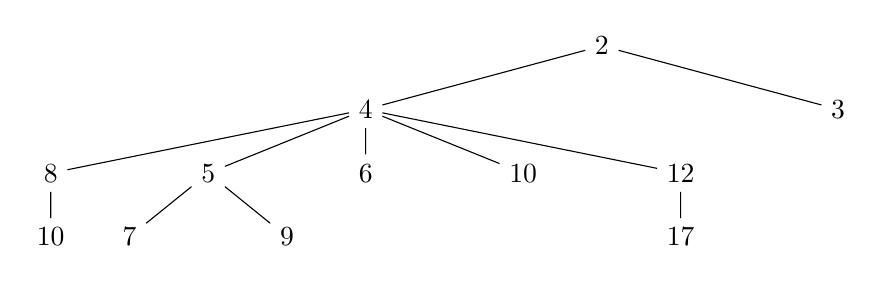
\begin{tikzpicture}[level 1/.style={sibling distance=60mm}, level 2/.style={sibling distance=20mm}, level distance=2.3em]
\node (2) {2}
  child {node (4) {4} %[sibling distance=20mm]
     child {node {8} child { node {10}}}
     child {node {5} child { node {7} } child { node {9}}}
     child {node {6} }
     child {node {10}}
     child {node {12} child { node {17}}}}
  child {node {3} };
\end{tikzpicture}
\end{center}
\end{frame}

\begin{frame}
\frametitle{Events and Finite-State Machines}
Remember: reactive, not proactive.\vfill
How can the application do what it wants?\vfill
\Large Use \alert{Finite-State Machines}!
\uncover<2>{
\begin{center}
\scalebox{0.6}{
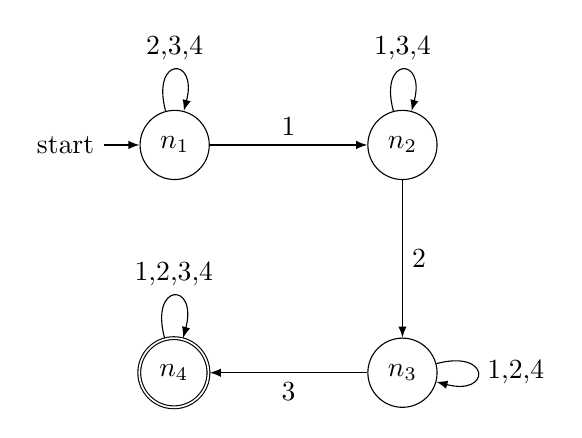
\begin{tikzpicture} [node distance=2cm, auto, every loop/.style={-latex},  every initial by arrow/.style={-latex}]

\node [state, initial] 	(n0){$n_1$};
\node [state] 			(n1) [right=of n0,]	{$n_2$};
\node [state]			(n2) [below=of n1]	{$n_3$};
\node [state, accepting](n3) [left=of n2]	{$n_4$};

\path[-latex] 
		(n0)edge				node	{1}		(n1)
			edge [loop above]	node	{2,3,4}	()
		(n1)edge				node	{2}		(n2)
			edge [loop above]	node	{1,3,4}	()
		(n2)edge				node	{3}		(n3)
			edge [loop right]	node	{1,2,4}	()
		(n3)edge [loop above]	node	{1,2,3,4}()
		;


\end{tikzpicture}}
\end{center}
}


\end{frame}

\begin{frame}
\frametitle{Where Events Come From}

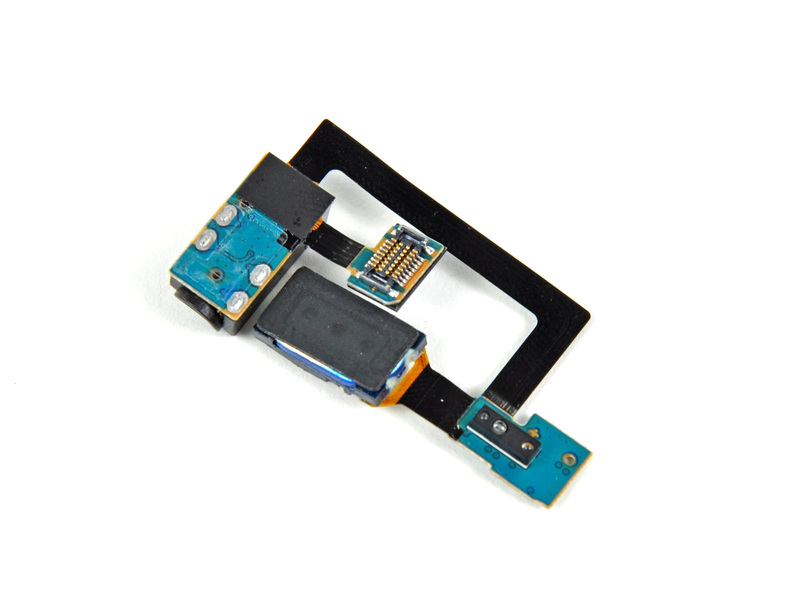
\includegraphics[width=.9\textwidth]{img/Galaxy_S_4G_037-small.jpg}

\vspace*{-1em}
\uncover<2>{Analog-to-Digital Converter. Then what?}

\end{frame}

\begin{frame}

\Huge
\begin{center}
``Are we there yet?''
\end{center}

\uncover<2>{\hfill --- example of \alert{polling}.}

\end{frame}

\begin{frame}
\frametitle{Polling}

\Large
Polling: processor requests readings from
the device at its convenience.  \vfill
``What is the current light level?''\vfill
(also known as ``passive synchronization'')

\end{frame}

\begin{frame}
\frametitle{When to Poll?}

\large
It depends:

\begin{itemize}
\item whenever convenient (occasional polling);
\item at fixed time intervals (periodic polling); or
\item constantly (tight polling).
\end{itemize}


\end{frame}

\begin{frame}
\frametitle{How to Get the Data}

\begin{center}
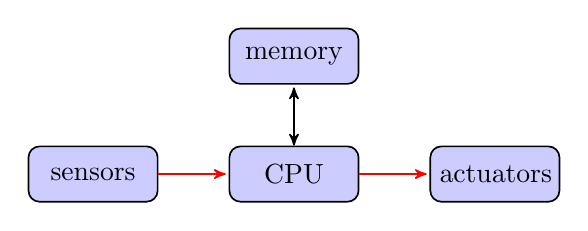
\begin{tikzpicture}[->,>=stealth',shorten >=1pt,auto,node distance=2.2cm,
                    semithick,initial text=]
  \node[bw]   (cpu)               {CPU};
  \node[bw, left of=cpu,xshift=-1em] (sensors) {sensors};
  \node[bw, right of=cpu,xshift=1em] (actuators) {actuators};
  \node[bw, above of=cpu,yshift=-2em] (memory) {memory};

  \path (cpu) edge[<->] node {} (memory)
        (sensors) edge[red] node {} (cpu)
        (cpu) edge[red] node {} (actuators);
\end{tikzpicture}
\end{center}

\large 
\vspace*{1em} What's the mechanism?

\uncover<2>{
\begin{itemize}
\item port-mapped I/O; or,\\[0.5em]
\item memory-mapped I/O
\end{itemize}
}


\end{frame}

\begin{frame}[fragile]
\frametitle{Port-mapped I/O: Special CPU Instructions}
The Intel ia32 processors provide special I/O instructions:\\[1em]
\begin{verbatim}
    outb   ax, 0x3f8
    inw    dx, ax
\end{verbatim}
~\\
May use a special bus, or set a specific signal on the bus.
\end{frame}


\begin{frame}
\frametitle{Memory-mapped I/O Example}
CPU just reads and writes to ``memory''.\\[1em]
\small
\begin{alltt}
 while (\alert{statusRegister} == 0x0000) \{\\
 \qquad // Do nothing until statusRegister changes value\\
 \}\\
 //  Read data that has changed from a dataRegister\\
 //  and store in memory\\
 incomingData = \alert{dataRegister};\\
\end{alltt}
~\\[1em] Devices listen on the bus and respond.
\end{frame}

\begin{frame}
\frametitle{Memory-mapped I/O Example}

\small
\begin{alltt}
 while (\alert{statusRegister} == 0x0000) \{\\
 \qquad // Do nothing until statusRegister changes value\\
 \}\\
 //  Read data that has changed from a dataRegister\\
 //  and store in memory\\
 incomingData = \alert{dataRegister};\\
\end{alltt}

This is a \emph{tight polling loop}.\\[1em]
\begin{itemize}
\item Expect the hardware specification to promise that statusRegister eventually changes 
due to an external event.
\item Data exchange occurs once device is ready: \alert{polling synchronization}.
\end{itemize}
\end{frame}

\begin{frame}
\frametitle{Interrupts: an alternative to polling}

\large
So far: processor controls when to read data from a device.\vfill
Instead: device may tell the processor when device is ready,
using an \alert{interrupt}.\vfill
This constitutes \alert{active synchronization}.
\end{frame}

\begin{frame}
\frametitle{How Interrupts Work}
Interrupt tells the processor: ``Something's happening!''\vfill

Upon receipt of an interrupt, the processor:
\begin{itemize}
\item stops what it's currently doing and saves its state;
\item starts executing pre-defined \alert{interrupt handler}, which:
\begin{itemize}
\item reads the event information; and
\item stores it somewhere accessible.
\end{itemize}
\item upon return from handler, resumes previous state.
\end{itemize}
\end{frame}

\begin{frame}
\frametitle{Inversion of Control: Without It}
Old ECE150 paradigm:\\[2em]

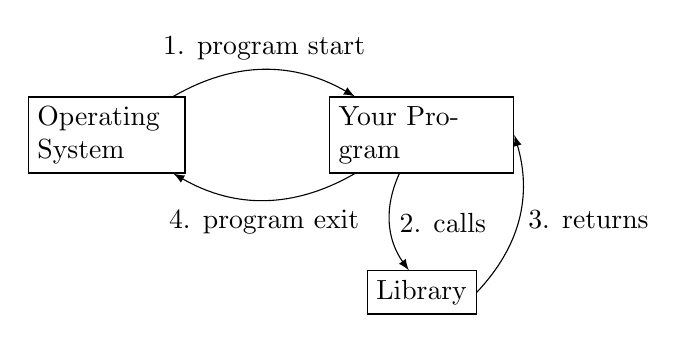
\begin{tikzpicture}
\path (0, 0) node[draw,text width=5em] (OS) { Operating System }
    +(4, 0) node[draw, text width=6em] (you) {Your Program};
\path<2-4> (4, -2) node[draw] (lib) {Library};

\path[->,bend left,>=latex] (OS) edge node[above] {1. program start} (you);
\path<4>[->,bend left,>=latex] (you) edge node[below] {4. program exit} (OS);
\path<2->[->,bend right,>=latex] (you) edge node[right] {2. calls} (lib);
\path<3->[->,bend right,>=latex] (lib.east) edge node[right] {3. returns} (you.east);
\end{tikzpicture}
\end{frame}

\begin{frame}
\frametitle{Inversion of Control: With It}
New event-driven ECE155 paradigm:\\[2em]

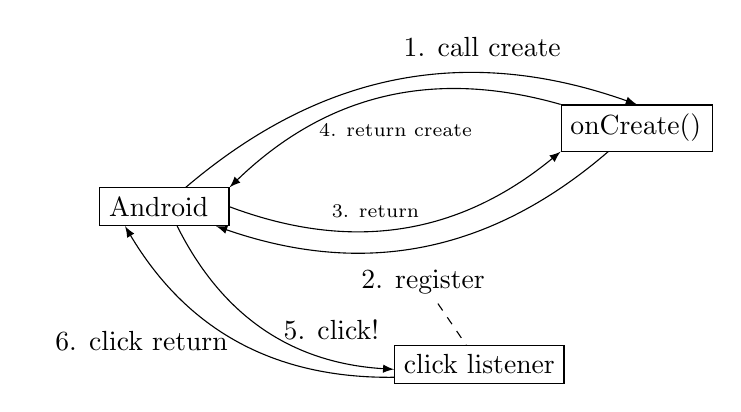
\begin{tikzpicture}
\path (0, 0) node[draw,text width=4em] (OS) { Android }
    +(6, 1) node[draw, text width=4.8em] (you) { onCreate() };
\path<2-> (4, -2) node[draw] (listener) {click listener};

\path[->,bend left,>=latex] (OS) edge node[above,yshift=0.5em, xshift=3em] {1. call create} (you.north);
\path<2->[->,bend left,>=latex] (you) edge node[below,name=reg,yshift=-.5em] {2. register} (OS);
\path<2->[dashed] (reg) edge (listener);
\path<3->[<-,bend left,>=latex] (you.south west) edge node[above,xshift=-1em,name=reg] {\scriptsize 3. return} (OS.east);
\path<4->[->,bend right,>=latex] (you.north west) edge node[above,at end,xshift=6em,yshift=1.5em] {\scriptsize 4. return create} (OS.north east);
\path<5->[->,bend right,>=latex] (OS) edge node[right] {~5. click!} (listener);
\path<6->[<-,bend right,>=latex] (OS.south)+(-0.5,0) edge node[left] {~~6. click return} 
                                 (listener)+(1,0);
\end{tikzpicture}
\end{frame}

\begin{frame}[fragile]
\frametitle{Behind the Scenes for Inversion of Control}
Android is running an event loop for each thread:
\begin{verbatim}
while (!done) {
 r <- fetch Runnable from Queue
 dispatch r
}
\end{verbatim}
This is a polling loop: in particular, a \structure{tight polling loop}, but which
goes to sleep waiting for the next event (in fetch).
\end{frame}

\begin{frame}
\frametitle{Miscellaneous: Real-Time Systems}

Must respond to an external event in a fixed amount of time. \\[1em]

This fixed amount of time is not necessarily small.
\begin{itemize}
\item may potentially be fixed and large.
\end{itemize}

Many embedded systems must satisfy real-time constraints.\\[1em]

In upper-year courses, you'll see both embedded systems and real-time
systems in more detail.

\end{frame}

\begin{frame}
\frametitle{Real-Time System Example}

\begin{center}
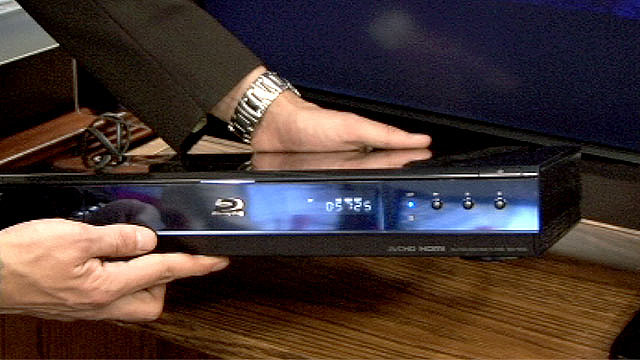
\includegraphics[width=.6\textwidth]{img/bluray}
\end{center}
\hfill {\small (credit {\tt digitaljournal.com}, from flickr)}

Blu-Ray player must:
\begin{itemize}
\item read compressed video data from a media disk;
\item decompress the video; and
\item output it to a HDMI interface,
\end{itemize}
all within a fixed amount of time, to avoid a degradation of video quality.


\end{frame}



\end{document}